%!TEX root=finmath2.tex

\chapter{Схема симуляции QE для модели Хестона}
\label{ch:qe}

В этом дополнении описана квадратично-экспоненциальная схема симуляции для модели Хестона (далее "--- \emph{схема QE}), которая является одной из наиболее эффективных схем для данной модели.
Она позволяет использовать существенно меньшее число промежуточных точек по сравнению со схемой Эйлера.
Схема QE была предложена в работе Л.~Андерсена \cite{Andersen08}.

\section{Описание схемы}
Рассмотрим модель Хестона, предполагая, что рисковый актив не выплачивает дивидендов, а безрисковая ставка равна нулю.
Будем симулировать процесс $(X_t, V_t)$, где $X_t = \ln S_t$.

Значения $(\hat X_{t_i}, \hat V_{t_i})$ будем генерировать последовательно по $i$. Предположим, что в момент $t_i$ значения известны, и покажем, как получить их в момент $t_{i+1}$.
Обозначим $\Delta t = t_{i+1} - t_i$.

Задача сводится к выбору случайного вектора $(\hat X_{t_{i+1}}, \hat V_{t_{i+1}})$ из условного распределения
\[
\Law (\hat X_{t_{i+1}}, \hat V_{t_{i+1}} \mid \hat X_{t_i}, \hat V_{t_i}).
\]
Разобьем ее на два шага: сначала получим значение $\hat V_{t_{i+1}}$ из распределения $\Law(\hat V_{t_{i+1}} \mid \hat V_{t_i})$, затем --- $\hat X_{t_{i+1}}$ из распределения $\Law(\hat X_{t_{i+1}} \mid \hat V_{t_i}, \hat X_{t_i}, \hat V_{t_{i+1}})$.

\medskip
\textit{Шаг 1.} Точное условное распределение $V_{t_{i+1}}$ имеет вид
\[
\Law(V_{t_{i+1}} \mid V_{t_i} = v ) 
  = \frac{\sigma^2(1-e^{-\kappa\Delta t})}{4\kappa} 
  \chi_d'^2\biggl(
    \frac{4\kappa e^{-\kappa\Delta t}}{\sigma^2(1-e^{-\kappa\Delta t})}v
  \biggr), \quad
d = \frac{4\theta\kappa}{\sigma^2},
\]
где $\chi_d'^2(\lambda)$ обозначает нецентральное распределение хи-квадрат%
\footnote{Для целого $d$ распределение $\chi_d'^2(\lambda)$ определяется как распределение суммы $(Z_1 + \mu_1)^2 + \ldots + (Z_d+\mu_d)^2$, где $Z_i$ --- независимые стандартные нормальные случайные величины, а $\mu_1^2 + \ldots + \mu_d^2 = \lambda^2$. Для произвольного $d>0$ оно задаётся соответствующей плотностью распределения.}
с $d>0$ степенями свободы и параметром нецентральности $\lambda > 0$.
Однако прямая симуляция из такого распределения вычислительно затруднительна.
Ключевая идея схемы QE состоит в том, чтобы использовать приближения.

Если значение $\lambda$ достаточно велико, то распределение $\chi_d'^2(\lambda)$ хорошо аппроксимируется квадратом нормального распределения.
Если же $\lambda$ мало, то оно хорошо приближается экспоненциальным распределением с добавлением дискретной массы в нуле.
Заметим, что в контексте симуляции $\hat V_{t_{i+1}}$ параметр нецентральности пропорционален значению $\hat V_{t_i}$.

Используя это наблюдение, будем строить $\hat V_{t_{i+1}}$ следующим образом:
\begin{itemize}
\item для больших $\hat V_{t_i}$ воспользуемся аппроксимацией
\begin{equation}
\label{qe:v-large}
\hat V_{t_{i+1}} = a(b+Z)^2,
\end{equation}
где $Z$ --- стандартная нормальная случайная величина, а $a,b$ --- параметры, зависящие от $\hat V_{t_i}$;

\item для малых $\hat V_{t_i}$ будем симулировать $\hat V_{t_{i+1}}$ из распределения с функцией распределения
\begin{equation}
\label{qe:v-small}
F(x) = p + (1-p)(1-e^{-\beta x}),
\end{equation}
где $p,\beta$ "--- параметры.
\end{itemize}

Параметры $a,b,p,\beta$ выбираются таким образом, чтобы у приближенного и настоящего распределения совпадали условное среднее и дисперсия.
А именно, обозначим
\[
\E(V_{t_{i+1}} \mid V_{t_i} = v) = m(v), \qquad 
\D(V_{t_{i+1}} \mid V_{t_i} = v) = s^2(v).
\]
Тогда верны следующие утверждения (доказательства можно найти в \cite{Andersen08}).

\begin{proposition}
Справедливы равенства
\begin{align*}
m(v) &= \theta + (v-\theta)e^{-\kappa \Delta t},\\
s^2(v) &= \frac{v \sigma^2 e^{-\kappa\Delta t}}{\kappa} 
  (1- e^{-\kappa\Delta t}) 
  + \frac{\theta\sigma^2}{2\kappa} (1-e^{-\kappa\Delta t})^2.
\end{align*}
\end{proposition}

\begin{proposition}
Пусть $\psi(v) = s^2(v)/m^2(v)$.
Тогда равенства
\[
\E(\hat V_{t_{i+1}} \mid \hat V_{t_i}=v) = m(v), \qquad
\D(\hat V_{t_{i+1}} \mid \hat V_{t_i}=v) = s^2(v)
\]
выполняются в следующих случаях:
\begin{enumerate}[topsep=0.5em]
\item если $\psi(v) \le 2$ и $\hat V_{t_{i+1}}$ вычисляется по формуле \eqref{qe:v-large} с параметрами
\[
b^2 = \frac{2}{\psi(v)} -1 + \sqrt{4-2\psi(v)}, \qquad a = \frac{m(v)}{1+b^2};
\]
\item если $\psi(v) \ge 1$ и $\hat V_{t_{i+1}}$ вычисляется по формуле \eqref{qe:v-small} с параметрами
\[
p = \frac{\psi(v)-1}{\psi(v)+1}, \qquad \beta = \frac{1-p}{m(v)}.
\]
\end{enumerate}
\end{proposition}

На практике используют правило: если $\psi(\hat V_{t_i}) \le 1.5$, то применяется аппроксимация \eqref{qe:v-large}; если $\psi(\hat V_{t_i}) \ge 1.5$, то аппроксимация \eqref{qe:v-small}. (Вместо числа $1.5$ можно выбрать любое значение между $1$ и $2$.)

\textit{Шаг 2.} Теперь рассмотрим симуляцию $\hat X_{t_{i+1}}$ из условного распределения $\Law (\hat X_{t_{i+1}} \mid \hat V_{t_i}, \hat X_{t_i}, \hat V_{t_{i+1}})$.
Из уравнений модели Хестона получаем
\begin{align*}
X_{t_{i+1}} &= X_{t_i} - \frac12 \int_{t_i}^{t_{i+1}} V_s ds 
  + \rho\int_{t_i}^{t_{i+1}} \sqrt{V_s} d W_s^{(1)} 
  + \sqrt{1-\rho^2} \int_{t_i}^{t_{i+1}} \sqrt{V_s} d W_s^{(2)},\\
V_{t_{i+1}} &= V_{t_i} + \kappa\theta\Delta t - \kappa\int_{t_i}^{t_{i+1}} V_s ds 
  + \sigma \int_{t_i}^{t_{i+1}} \sqrt{V_s} d W_s^{(1)}.
\end{align*}
Выражая стохастический интеграл из второго уравнения и подставляя его в первое, получаем
\begin{multline*}
X_{t_{i+1}} = X_{t_i} 
  + \frac{\rho}{\sigma} (V_{t_{i+1}} - V_{t_i} - \kappa\theta\Delta t) \\
+ \biggl(\frac{\kappa\rho}{\sigma} - \frac12\biggr) 
  \int_{t_i}^{t_{i+1}} V_s ds 
+ \sqrt{1-\rho^2} \int_{t_i}^{t_{i+1}} \sqrt{V_s} d W_s^{(2)}.
\end{multline*}
Аппроксимируем интегралы, взяв значение подынтегральных процессов в левой точке отрезка интегрирования:
\[
\int_{t_i}^{t_{i+1}} V_s ds \approx V_{t_i} \Delta t, \qquad
\int_{t_i}^{t_{i+1}} \sqrt{V_s} d W^{(2)}_s \approx \sqrt{V_{t_i} \Delta t} \Delta W_{t_{i+1}}^{(2)},
\]
где в качестве $\Delta W_{t_{i+1}}^{(2)}$ нужно взять нормальную случайную величину с нулевым средним и дисперсией $\Delta t$, не зависящую от значений $\hat X_{t_i}$, $\hat V_{t_i}$, $\hat V_{t_{i+1}}$.

Таким образом, значение  $\hat X_{t_{i+1}}$ получается по формуле
\[
\hat X_{t_{i+1}} = \hat X_{t_i} + K_0 + K_1 \hat V_{t_i} 
+ K_2 \hat V_{t_{i+1}} + \sqrt{K_3 \hat V_{t_i}} \,\Delta W_{t_{i+1}}^{(2)},
\]
где коэффициенты равны
\[
K_0 = -\frac{\rho\kappa\theta}{\sigma} \Delta t, \quad 
K_1 = \biggl(\frac{\kappa\rho}{\sigma} - \frac12\biggr)\Delta t - \frac{\rho}{\sigma}, \quad
K_2 = \frac{\rho}{\sigma}, \quad
K_3 = 1-\rho^2.
\]

\begin{remark}
В приведённой форме схема QE, вообще говоря, не обладает мартингальным свойством (\te\ равенством $\E(\hat S_{t_{i+1}} \mid \F_{t_i}) = \hat S_{t_i}$).
В работе \cite{Andersen08} описан вариант схемы QE с \emph{мартингальной поправкой}, однако при его использовании необходимо пересчитывать коэффициент $K_0$ на каждом шаге.
\end{remark}

\section{Сравнение со схемой Эйлера}
На рис.~\ref{qe:f:comparison} представлено сравнение точности схем QE и Эйлера.
Графики показывают отклонение подразумеваемой волатильности, когда цены опционов вычисляются по методу \mc, от истинной подразумеваемой волатильности. 
В качестве параметров модели взяты $V_0=0.1,\kappa=1, \theta=0.1,\sigma=1.5,\rho=-0.6$; время исполнения опционов $T=1$.

Видно, что схема QE дает достаточно точный результат даже для малого количества промежуточных точек, в то время как схеме Эйлера требуется гораздо большее их количество для достижения приемлемой точности.

\begin{figure}[h]
\centering
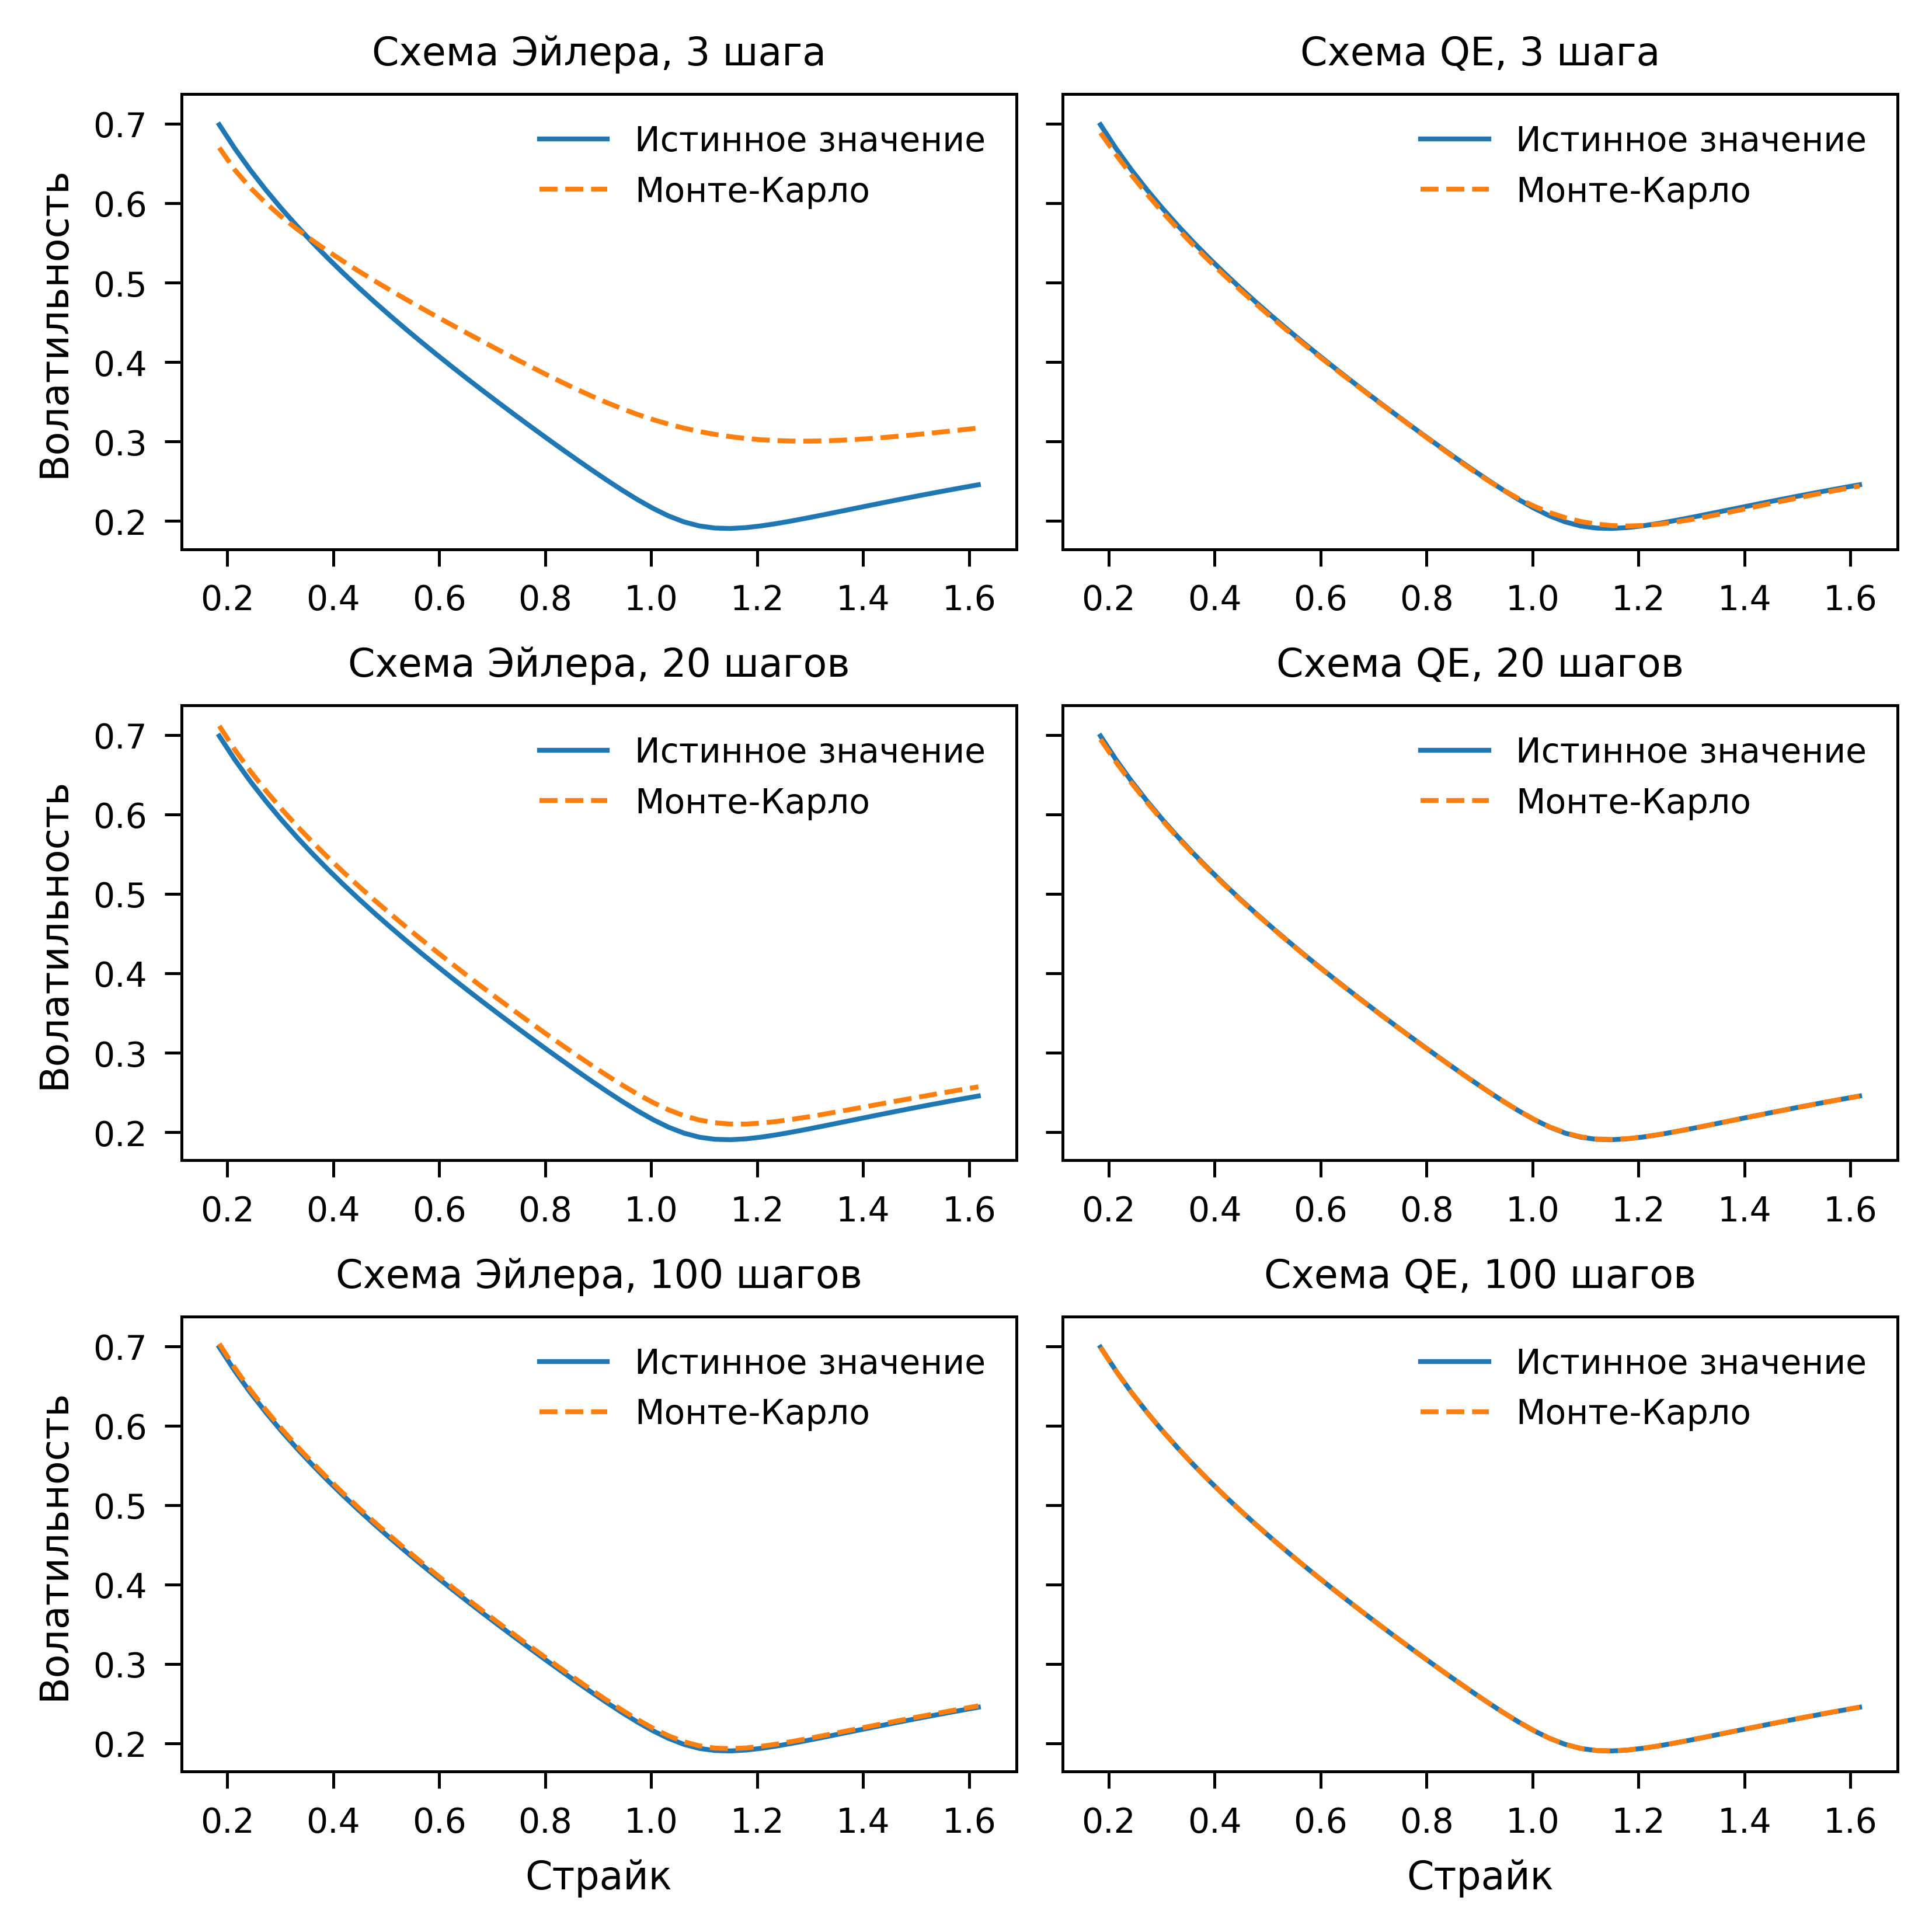
\includegraphics{pic/heston-qe.png}  
\caption{Сравнение точности схемы Эйлера и схемы QE.}
\label{qe:f:comparison}
\end{figure}
